\chapter{Herramientas}

La complejidad que acarrea el uso de aplicaciones distribuidas hace necesario el uso de herramientas que permitan el desarrollo de forma cómoda del propio sistema, su uso posterior como herramienta de prueba de aplicaciones distribuidas y por último, facilitar el aprendizaje de algoritmos y herramientas distribuidas.

Muchas de las aplicaciones distribuidas utilizadas incluyen varias herramientas para facilitar su uso. Sin embargo estas soluciones suelen ser diseñadas para el propósito específico de dicha aplicación, y son difíciles de adaptar a otros contextos. Debido a esta carencia, se han creado varias herramientas propias que permiten aprovechar al máximo este sistema.

\section{MarcoPolo, el protocolo de descubrimiento de servicios}

Uno de los problemas típicos a la hora de crear un sistema distribuido es la localización de cada uno de los nodos que lo conforman. Soluciones como servicios de nombres (DNS) permiten crear estructuras jerárquicas donde cada nodo está identificado por un nombre previamente conocido. También existen protocolos inspirados en este como mDNS (\textit{Multicast Domain Name Service}) donde la necesidad de un servidor de nombres desaparece, y los nodos son capaces de encontrarse entre ellos mediante multicast. Otras alternativas como Bonjour, Avahi o AppleTalk (ya descontinuado) también han sido evaluadas. %TODO

Sin embargo, estas y otras soluciones similares no responden a una de las necesidades básicas del sistema a construir: la condición de que la información que conoce cada nodo sobre el resto en el arranque del sistema es nula. Si bien con mDNS evitamos contar con un servidor de nombres, debemos conocer el nombre de cada máquina o esta debe anunciarse en la red antes de poder estar disponible (mDNS Probing). Dicho inconveniente se suma al hecho de que DNS y protocolos similares son creados con el único propósito de resolver la correspondencia nombre - dirección de red de un equipo, y son difícilmente extensibles a otro tipo de aplicaciones. Además, la mayoría de los protocolos asumen que la información de un nodo presente de una red local es de interés para el resto de nodos de la red, lo cual dificulta la independencia de un conjunto de equipos frente al resto.

Una de las piezas clave del sistema consiste en la escalabilidad del mismo en tiempo real: no es necesario conocer qué nodos participan en el sistema hasta que no se vayan a utilizar. Además, se pretende optimizar al máximo cada uno de los nodos del sistema por separado, por lo que dedicar uno de ellos como ``autoridad'' frente a la que el resto de nodos se registren y esta actúe posteriormente como nodo coordinador y ``resolver'' supone una dedicación de recursos innecesaria y que dificulta la escalabilidad del sistema. Además, la gestión del espacio de direcciones de la red en la que se integra el sistema no es gestionado por este y además es compartido con una gran cantidad de equipos adicionales. Esto implica que las direcciones de cada nodo son asignadas por un servidor DHCP (\textit{Dynamic Host Configuration Protocol}) sobre el que no se tiene control, y cuyas direcciones son asignadas para intervalos de tiempo pequeños\footnote{Durante el desarrollo del sistema se observa que las direcciones son asignadas por periodos de tiempo pequeños y no suelen repetirse a menos que dicha dirección no haya sido asignada anteriormente, fenómeno que suele darse con bastante frecuencia.}. %TODOEsto implica que no es posible contar con un nodo coordinador sin un espacio de nombres anteriormente definido.
Por otro lado, la clave de este sistema no la constituye la disponibilidad de un nodo, sino las aplicaciones distribuidas que pueden utilizarse en el mismo (de ahora en adelante denominaremos a estas ``servicios''). Un nodo puede contar con un conjunto de servicios diferente al de sus vecinos, y por tanto colaborará en unas tareas y en otras no en virtud de dicha disponibilidad. Este requisito no es satisfecho por la mayoría de los sistemas anteriormente mencionados.

Motivada por esta serie de características surge la necesidad de crear un pequeño protocolo de descubrimiento de nodos basado principalmente en los servicios que dichos nodos pueden (y desean) ofrecer al conjunto de la malla. Además, siendo uno de los objetivos funcionales del sistema el aprovechamiento del mismo como herramienta didáctica, surge la necesidad de que dos conjuntos de nodos puedan trabajar en la misma red de forma independiente. Como aproximación para satisfacer estas necesidades surge el procolo de descubrimiento de servicios \textbf{MarcoPolo}

\subsection{MarcoPolo: Introducción}

MarcoPolo es un protocolo de descubrimiento de servicios cuya dinámica y nombre se inspiran en el juego homónimo, en el cual uno de los integrantes debe encontrar al resto privado de visión mediante ecolocalización (gritando la palabra clave ``Marco'', cuya respuesta por parte del resto de jugadores es ``Polo''). El protocolo se compone de dos roles claramente diferenciados (y prácticamente independientes aún siendo ejecutados en el mismo nodo): \textbf{Marco}, encargado de enviar consultas a la red y \textbf{Polo}, que emite una respuesta a dichos comandos y gestiona la información de cada nodo.

Con el objetivo de posibilitar la coexistencia de varias ``mallas'' de nodos independientes (donde los servicios ofrecidos por un nodo únicamente sean conocidos y consecuentemente aprovechables por el resto de sus vecinos) a la vez que las consultas son realizadas a todos los integrantes sin necesidad de conocer su identificador en la red (dirección a nivel de red o enlace, nombre \textit{DNS}) se utilizan mensajes uno-a-muchos, conocidos generalmente con el nombre \textit{multicast}, donde cada una de las \textit{mallas} se comunicará con el resto de integrantes de la misma a través de un grupo preestablecido (o consensuado por dichos nodos).

El protocolo consiste en una serie de mensajes (a partir de ahora denominados \textit{comandos}) que contienen las consultas sobre la información de uno o varios servicios, nodos o información sobre la propia \textit{malla} que un nodo desee conocer, así como la respuesta a dichas consultas. Dichos mensajes son enviados como cadenas de texto que almacenan la información en estructuras de datos JSON (\textit{JavaScript Object Notation}) debido a la gran legibilidad de estas por humanos y la gran cantidad de herramientas disponibles para su creación y procesado.

\subsection{Arquitectura en detalle}

\subsection{Comandos}

Los comandos de MarcoPolo constituyen las primitivas del protocolo. Actualmente se cuenta con las siguientes primitivas y las correspondientes respuestas:

\begin{table}[c]
\begin{tabular}{|p{1.5cm}|p{1cm}|p{3cm}|p{3cm}|p{3cm}|p{1.5cm}|}
\hline
Nombre & Agente emisor & Función & Información & Respuesta esperada & Protocolo y puerto\\ \hline
\textbf{Marco} & Marco & Descubrir todos los nodos presentes en la \textit{malla} & Únicamente se incluye el nombre del comando & Un comando \textit{Polo} por cada nodo disponible en la red, incluyendo como parámetros opcionales información sobre el nodo o \textit{ninguna} si no existe ningún nodo disponible. & UDP \textit{multicast} al puerto 1338.\\ \hline
\textbf{Polo} & Polo & Informar a un nodo de la existencia del emisor & Información sobre el nodo opcional (servicios disponibles, información sobre el nodo o la instancia de Polo\dots) & \textit{Ninguna} &  UDP \textit{unicast} al puerto efímero del mensaje de pregunta.\\ \hline
\textbf{Request-For} & Marco & Conocer todos los nodos que ofrecen un servicio identificado por su nombre único en el sistema & Identificador unívoco del servicio a descubrir & \textbf{OK} con información opcional sobre el nodo o el servicio & UDP \textit{multicast} al puerto 1338.\\ \hline
\textbf{OK} & Polo & Comando utilizado para emitir una respuesta a una petición, siendo la información de interés contenida en los parámetros de respuesta. & Respuesta a un comando con la información solicitada & \textit{Ninguna} & UDP \textit{unicast} al puerto efímero de la pregunta.\\ \hline
\textbf{Services} & Marco & Descubrir todos los servicios ofrecidos por un nodo & No se envía información adicional con el comando & \textbf{OK} con una lista de los identificadores del servicio o \textit{ninguna} si el nodo no está en la red. & UDP \textit{unicast} al puerto 1338.\\ \hline
\end{tabular}
\end{table}

\subsection{Esquemas de comunicación}

\subsubsection{Comando \textbf{Marco}}

\begin{figure}[h]
\centering
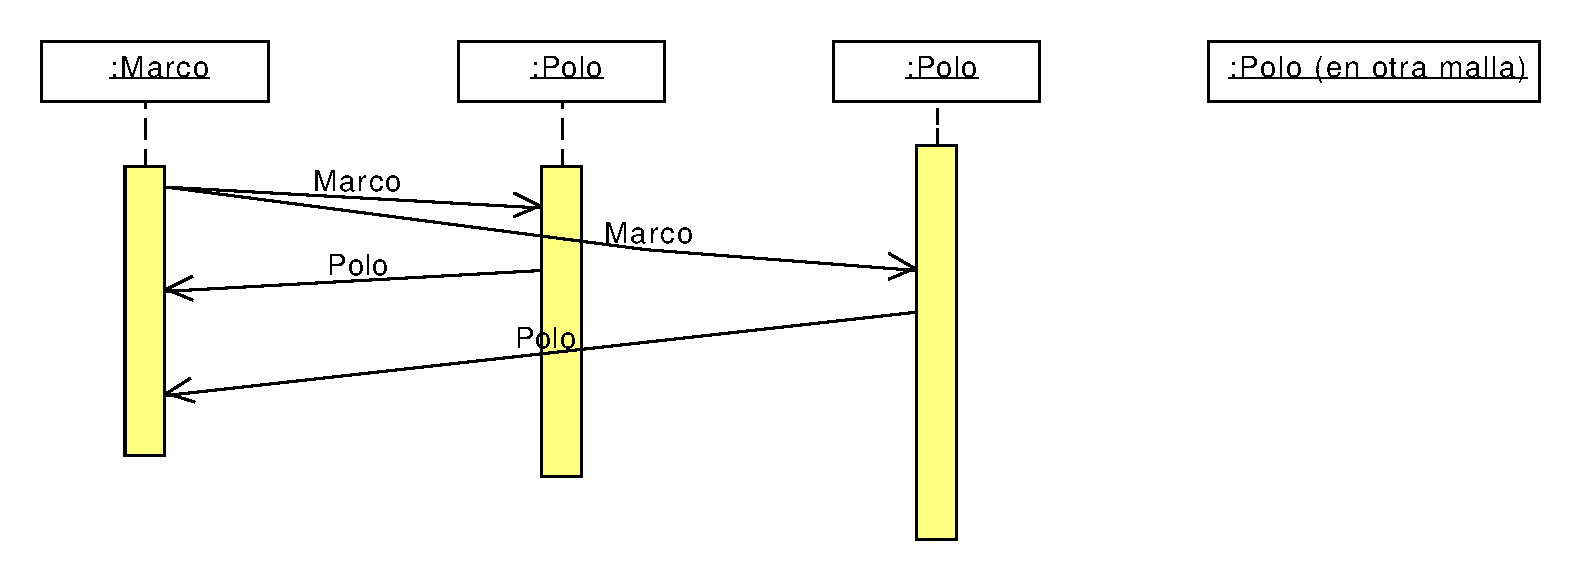
\includegraphics[width=0.8\textwidth]{Diagrams/Sequence/marco}
\caption{Interacción al enviar el comando \textbf{Marco}}
\label{fig:secuencia_marco}
\end{figure}

El comando Marco se envía al grupo \textit{multicast} definido en la configuración de la instancia local de \textbf{Marco}. Los nodos suscritos a dicho grupo (aquellos que pertenecen a la ``malla'') reciben el mensaje y emiten una respuesta \textbf{Polo}. Debido a la falta de una conexión entre los nodos (debido a que todos los mensajes son intercambiados utilizando el protocolo UDP) se fija un tiempo de espera de respuesta, durante el cual se reciben y acumulan todas las respuestas. Al final dicho tiempo de espera, se retornan los resultados y el resto de respuestas son ignoradas.

\section{Aplicaciones construidas sobre MarcoPolo}
 

%\includegraphics{Chapter3/ScreenShot.png}